% -*- TeX:UTF-8 -*-
%%
%% KAIST 학위논문양식 LaTeX용 (ver 0.5) 예시
%%
%% @version 0.4
%% @author  채승병 Chae,Seungbyung (mailto:chess@kaist.ac.kr)
%% @date    2004. 11. 12.
%%
%% @requirement
%% teTeX, fpTeX, teTeX 등의 LaTeX2e 배포판
%% + 은광희 님의 HLaTeX 0.991 이상 버젼 또는 홍석호 님의 HPACK 1.0
%% : 설치에 대한 자세한 정보는 http://www.ktug.or.kr을 참조바랍니다.
%%
%% @note
%% 기존에 널리 쓰여오던 차재춘 님의 학위논문양식 클래스 파일의 형식을
%% 따르지 않고 전면적으로 다시 작성하였습니다. 논문 정보 입력부분에서
%% 과거 양식과 다른 부분이 많으니 아래 예시에 맞춰 바꿔주십시오.
%%
%%
%% @acknowledgement
%% 본 예시 논문은 물리학과 박사과정 김용현 님의 호의로 제공되었습니다.
%%
%% -------------------------------------------------------------------
%% @information
%% 이 예제 파일은 hangul-ucs를 사용합니다. UTF-8 입력 인코딩으로
%% 작성되었습니다. hlatex의 hfont는 이용하지 않습니다. --2006/02/11
%% 본 템플릿은 전산학부 김민혁 교수에의해서 버그 수정되었습니다. -- 2016/11/25

% @class kaist.cls
% @options [default: doctor, korean, final]
% - doctor: 박사과정 | master : 석사과정
% - korean: 한글논문 | english: 영문논문
% - final : 최종판   | draft  : 시험판
% - pdfdoc : 선택하지 않으면 북마크와 colorlink를 만들지 않습니다.


\documentclass[master,english,final]{kaist-ucs}

\newcommand{\documenttype}{Master Thesis}
\newcommand{\thesistitle}{Portable Ultrasound System for Blood Velocity Estimation}
\newcommand{\thesissubtitle}{Project Report}

\newcommand{\thesisauthor}{Jeppe Hinrichs} % Your name :)
\newcommand{\studentnumber}{s163555}
\newcommand{\thedate}{April, 2023} % For example "June, 2019"

\newcommand{\dtudepartment}{DTU Department of Electrical Engineering}
\newcommand{\dtudepartmentdescriber}{DTU Elektro, Institut for Elektroteknologi}
\newcommand{\dtuorg}{Technical University of Denmark}
\newcommand{\dtuaddressI}{Ørsteds Plads, Building 348}
\newcommand{\dtuaddressII}{2800 Kgs. Lyngby}
\newcommand{\dtudepartmentwebsite}{www.elektro.dtu.dk}

\newcommand{\kaistdepartment}{KAIST EE}
\newcommand{\kaistdepartmentdescriber}{한국과학기술원 전기 및 전자공학부}
\newcommand{\kaistorg}{한국과학기술원}
\newcommand{\kaistaddressI}{E3-2, 291 대학로 유성구}
\newcommand{\kaistaddressII}{34141 대전}
\newcommand{\kaistdepartmentwebsite}{www.ee.kaist.ac.kr}

\newcommand{\projectstartdate}{\formatdate{1}{10}{2022}}
\newcommand{\projectenddate}{\formatdate{24}{5}{2023}}
\newcommand{\projectcredits}{30 ECTS / 9 credits}
\newcommand{\degreename}{Electrical Engineering}
\newcommand{\degreetype}{Master of Science}
% If you want make pdf document (include bookmark, colorlink)
%\documentclass[doctor,english,final,pdfdoc]{kaist-ucs}

% kaist.cls 에서는 기본으로 dhucs, ifpdf, graphicx 패키지가 로드됩니다.
% 추가로 필요한 패키지가 있다면 주석을 풀고 적어넣으십시오,
%\usepackage{...}

\usepackage{parskip}        % Package to tweak paragraph skipping (instead of indents a small skip is added after every paragraph)
\usepackage{titlesec}
%\usepackage{tikz}           % Package for drawing
\usepackage{pgfplots}       % Package for creating graphs and charts
\usepackage{xcolor}         % Package for defining DTU colours to be used
\selectcolormodel{natural}
\usepackage{ninecolors}
\selectcolormodel{rgb}
\usepackage{amsmath}        % For aligning equations among other
\usepackage{mathtools}		% Extensible symbols, brackets, arrows, etc
\usepackage{xfrac}			% More modern than nicefrac
\usepackage{listings}       % Package for inserting code, (before cleveref)
\usepackage[chapter]{minted}
%\setminted{autogobble,linenos=true,breaklines,labelposition=all}
\usepackage[most, minted]{tcolorbox}
%\usepackage[most]{tcolorbox}
%\tcbuselibrary{listings, breakable, skins}
\PassOptionsToPackage{hyphens}{url} % Ability to line break urls at hyphens
\usepackage{cleveref}       % improved cross referencing
\usepackage{textcomp}       % \textdegree = °C and other useful symbols
\usepackage{caption}        % better captions
\usepackage{subcaption}     % for subfigures
\usepackage[autostyle=true]{csquotes}       % For biblatex with babel
\usepackage[backend=biber,style=ieee,abbreviate=true,dateabbrev=false,alldates=long,sorting=ynt,dashed=false,block=space,mincitenames=1,maxcitenames=1,maxbibnames=9,backref=false]{biblatex} % Package for bibliography (citing)
\bibliography{bib_bibertool.bib}

% Tables
\usepackage{float}          % floating figures in correct places
\usepackage{adjustbox}				% Adjust table widths (?)
\usepackage{nth}			% 1st, 2nd, etc
\usepackage{tabularray}		% latex3 tables
\UseTblrLibrary{booktabs,siunitx,varwidth}

% Extras
\usepackage[automake=immediate,toc, % Abbreviations and glossary lists
abbreviations,
postdot,
hyperfirst=true,
nopostdot=true,
nonumberlist=true,
nowarn,
]{glossaries-extra}
\usepackage{glossary-longextra} % Long booktabs table style
\usepackage[numbib]{tocbibind} % Lists of... in toc
%\usepackage{tocloft}		% Customising toc
%\usepackage{calc}           % Adds ability for latex to calculate (3pt+2pt)
\usepackage{blindtext}
\usepackage{graphicx}
\graphicspath{{Figures/}} %Setting the graphicspath
\usepackage{svg}
\usepackage[colorinlistoftodos]{todonotes} % Margin coloured todonotes
\usepackage{pdflscape}
% Drawing
\usepackage{tikz}					% Create graphics
\usetikzlibrary{arrows.meta,chains,backgrounds,positioning,fit,petri,automata,quotes}
\usepackage{xstring}				% For manipulating strings. Required by CircuiTikZ
\usepackage[american,arrowmos,nooldvoltagedirection]{circuitikz}	% Create circuit graphics (using TikZ)

\usepackage[verbose=silent,protrusion=true,expansion=true,final,babel]{microtype} % Better text appearance
\usepackage{hyphenat}			% Prevent hyphenation by \nohyphens{text}
\usepackage{pgfgantt}


% @command title 논문 제목(title of thesis)
% @options [default: (none)]
% - korean: 한글제목(korean title) | english: 영문제목(english title)
\title[korean] {혈류 속도 예측을 위한 휴대용 초음파 시스템}
\title[english]{Portable ultrasound system for blood velocity estimation}

% @note 표지에 출력되는 제목을 강제로 줄바꿈하려면 \linebreak 을 삽입.
%       \\ 나 \newline 등을 사용하면 안됩니다. (아래는 예시)
%
%\title[korean]{탄소 나노튜브의 물리적 특성에 대한\linebreak 이론 연구}
%\title[english]{Theoretical study on physical properties of\linebreak
	%                carbon nanotubes}
%
% If you want to begin a new line in cover, use \linebreak .
% See examples above.
%


% @command author 저자 이름
% @param   family_name, given_name 성, 이름을 구분해서 입력
% @options [default: (none)]
% - korean: 한글이름 | chinese: 한문이름 | english: 영문이름
% 한문 이름이 없다면 빈 칸으로 두셔도 됩니다.
%
%
% If you are a foreigner , write your name in korean or your korean name.
% If you can't write native character, you can make the chinese blank empty
% Write as follow
% \author[korean]{family name in korean}{given name in korean}
% \author[chinese]{family name in your native language}{given name in your native language}
% \author[english]{family name in english}{given name in english}
%
\author[korean]{힌릭스}{예페}
\author[korean2]{힌릭스}{예페}   %이름을 붙여 써 주시기 바랍니다.
\author[chinese]{}{}
\author[english]{Hinrichs}{Jeppe}

% @command advisor 지도교수 이름 (복수가능)
% @usage   \advisor[options]{...한글이름...}{...영문이름...}{signed|nosign}
% @options [default: major]
% - major: 주 지도교수  | coopr: 공동 지도교수
\advisor[major]{이 현 주}{Hyunjoo Lee}{signed}
\advisor[major2]{}{Fafoutis Xenofon}{signed}    %한글 성과 한글 이름을 모두 붙여 써 주시기 바랍니다.
\advisorinfo{Professor of Electrical Engineering} %제출승인서에 들어가는 교수님 정보, advisor's information
%\advisor[coopr]{홍 길 동}{Gil-Dong Hong}{nosign}
%\advisor[coopr2]{홍길동}{Gil-Dong Hong}{nosign}    %한글 성과 한글 이름을 모두 붙여 써 주시기 바랍니다.
%
% 지도교수 한글이름은 입력하지 않아도 됩니다.
% You may not input advisor's korean name
% like this \advisor[major]{}{Chang, Kee Joo}{signed}
%


% @command department {학과이름}{학위종류} - 아래 규칙에 따라 코드를 입력
% @command department {department code}{degree field}
%
% department code
% 2. 석박사학위논문 작성 및 제출요령 4쪽 ~ 5쪽 참고
% 또는 kaist-ucs.cls 의 % @command department 참고

% science: 이학 | engineering: 공학 | business : 경영학
% 박사논문의 경우는 학위종류를 입력하지 않아도 됩니다.
% If you write Ph.D. dissertation, you cannot input degree field.
% The third parameter : a | b | c
% a: 소속된 학과만 쓰는 옵션 (학과에만 소속되어 있는 경우에는 무조건 a를 선택해야 함)
% b: 학과 아래의, 프로그램이나 학제전공에 소속되어 있을 경우에 학과와 프로그램을 함께 쓰는 옵션
% c: 학과 아래의, 프로그램이나 학제전공에 소속되어 있을 경우에 학과를 쓰지 않고 프로그램이나 학제전공의 이름만 쓰는 옵션
%
% a: it represents only the name of department. (if you aren't in the program under the department, must choose a)
% b: it represents the names of department and the program that is under the department (consider this when you are in the program not only department)
% c: it represents only the name of program that is under the department (consider this when you are in the program not only department)
\department{EE}{engineering}{a}

% @command referee 심사위원 (석사과정 3인, 박사과정 5인)
\referee[1]{이 현 주}
\referee[2]{Fafoutis Xenofon}
\referee[3]{제 민 규}
\referee[4]{Zsurzsan Tiberiu Gabriel}
\referee[5]{Micconi Laura}
% \referee[5] {Barack Obama}
% Of course english name is available

% @command approvaldate 지도교수논문승인일
% @param   year,month,day 연,월,일 순으로 입력
\approvaldate{2023}{6}{15}

% @command refereedate 심사위원논문심사일
% @param   year,month,day 연,월,일 순으로 입력
\refereedate{2023}{6}{15}

% @command gradyear 졸업년도
\gradyear{2023}

% 본문 시작
\makeglossaries

\begin{document}


	% 앞표지, 속표지, 학위논문 제출승인서, 학위논문 심사완료 검인서는
	% 클래스 옵션을 final로 지정해주면 자동으로 생성되며,
	% 반대로 옵션을 draft로 지정해주면 생성되지 않습니다.

	% 논문 서지, 초록, 핵심 낱말, 영문 초록, 영어 핵심 낱말 (Information of thesis, abstract in korean, keywords in korean, abstract in english, keywords in english)
	\thesisinfo
	%% Letters of abstract in korean must be less than 500 and words of abstract in english must be less than 300.
	%% Number of keywords must be less than 6.
	%% Don't write english letters in the abstract in korean.
	\begin{summary}
		초음파 이미징은 혈류 측정을 수행하는 중요한 방법이다. 이 보고서는 그러한 초음파 혈 류 측정 시스템의 설계, 구현과 분석을 담고 있다. 초음파 혈류 측정 시스템은 Xilinx Zynq	7000 SoC 라는 중앙 제어 시스템을 기반으로 자체 제작된 아날로그 프론트 엔드를 구현하	기 위한 다양한 초음파 펄스 및 타이밍 신호를 발생시킨다. 또한, 이 시스템은 직교 복조를 이용하여 복조된 도플러 주파수를 얻는다. 모듈 단위로 시스템을 테스트하였으나 시간 제 약으로 인해 전체를 테스트하지는 못하였다.
	\end{summary}

	\begin{Korkeyword}
		인지 무선 통신, 협력 통신, 중계, 전 이중, 동시 송수신
	\end{Korkeyword}


	\begin{abstract}
		For blood flow estimation, ultrasound imaging is an important tool. This project report outlines the design, implementation, and analysis of such ultrasound blood velocity estimator. The design is based off a central control system on a Xilinx Zynq 7000 SoC for generating ultrasound pulses and the various timing signals needed for operating the custom designed analogue front-end. The chosen design topology uses a pulsed-wave design with quadrature demodulation to obtain the Doppler frequency. The system was module tested, but was not fully end-to-end tested on a physiological simulator due to time constraints.
	\end{abstract}

	\begin{Engkeyword}
		Cognitive radio, cooperation communication, relay, full-duplex, simultaneous transmission and reception
	\end{Engkeyword}


	\addtocounter{pagemarker}{1}                 % 백색별지분을 고려
	\newpage



	% 목차 (Table of Contents) 생성
	\tableofcontents

	% 표목차 (List of Tables) 생성
	\listoftables

	% 그림목차 (List of Figures) 생성
	\listoffigures

	% 위의 세 종류의 목차는 한꺼번에 다음 명령으로 생성할 수도 있습니다.
	%\makecontents

	%% 이하의 본문은 LaTeX 표준 클래스 report 양식에 준하여 작성하시면 됩니다.
	%% 하지만 part는 사용하지 못하도록 제거하였으므로, chapter가 문서 내의
	%% 최상위 분류 단위가 됩니다.
	%% You cannot use 'part'

	\chapter{Introduction} \label{cha:introduction} %\thispagestyle{main}
The progress of diagnostic imaging has advanced significantly during the \nth{20} century. As the cost of high-speed computational systems has grown increasingly accessible, so has the use of medical imaging become prominent. Millions of people have potentially been spared painful exploratory surgery through non-invasive diagnostic imaging. Thus, lives can be saved by early diagnosis and intervention through medical imaging. Advancements in scientific visualisation have in turn generated more complex data-sets of increased size and quality. The four major technologies used are \gls{us}, X-ray, \gls{ct}, and \gls{mri}. Each technology has distinct advantages and disadvantages in biomedical imaging, and thus each is still relevant for modern medicine. \Cref{tab:1_imagingmodalities} contains a comparison and summary of the various fundamental diagnostic imaging modalities.

\begin{table}[htbp]
	\centering
	\begin{talltblr}[
	caption = {Comparison of medical imaging modalities \cite{Szabo_UltrasoundBook_2}},
	entry = {Comparison of medical imaging modalities},
	label = {tab:1_imagingmodalities},
	note{a} = {Frequency and axially dependent.},
	note{b} = {Frequency dependent.},
	note{c} = {Fluoroscopy limited.},
	note{$\dag$} = {Typical: 45 minutes, fastest: Real-time (\glsxtrshort{low-res}).},
	]{
		%colspec = {Q[l,t]Q[l,t]Q[l,t]Q[l,t]Q[l,t]},
		%colspec = {Q[jQQQQ},
		row{1} = {guard, m, font=\small\bfseries},
	}
	\toprule
	\textbf{Modality} & \textbf{Ultrasound} & \textbf{X-ray} & \textbf{CT} & \textbf{MRI} \\ \midrule
	Topic             & {Longitudinal,\\shear,\\mechanical\\properties} & {Mean X-ray\\tissue\\absorption} & {Local tissue\\X-ray absorbtion} & {Biochemistry \\(\textit{T1} and \textit{T2})}    \\
	Access            & {Small\\windows\\adequate} & {2 sides\\needed} & {Circumferential\\around\\body} & {Circumferential\\around\\body} \\
	{Spatial\\resolution} & {\qty{0.2}{\milli\meter} to\\\qty{3}{\milli\meter}\TblrNote{a}} & $\sim \qty{1}{\milli \meter}$ & $\sim \qty{1}{\milli \meter}$ & $\sim \qty{1}{\milli \meter}$ \\
	Penetration     & {\qty{3}{\centi\meter} to\\\qty{25}{\centi\meter}\TblrNote{b}} & Excellent  & Excellent & Excellent \\
	Safety          & Excellent & {Ionizing\\radiation}      & {Ionizing\\radiation} & Very good \\
	Speed           & Real-time & Minutes & 20 minutes & Varies\TblrNote{$\dag$} \\
	Cost            & \$ & \$ & \$\$ & \$\$\$ \\
	Portability     & Excellent & Good & Poor & Poor \\
	{Volume\\coverage} & {Real-time\\3D volumes,\\improving} & 2D & {Large 3D\\volume} & {Large 3D \\volume} \\
	Contrast        & {Increasing\\(shear)} & Limited & Limited & {Slightly\\flexible} \\
	Intervention    & {Real-time\\3D increasing} & No\TblrNote{c} & No & Yes, limited \\
	Functional      & {Functional\\ultrasound} & No & No & fMRI \\
	\bottomrule
\end{talltblr}
\end{table}

Between 2004 and 2016\todo{Fix end year}, medical imaging has been reported to have been performed more than 5 billion times \cite{Picano2004}. Later numbers from 2011 show a general doubling and in particular, a tenfold increase in ultrasound examinations between 2000 and 2011 \cite{Szabo_UltrasoundBook_2}. Recent data reveal that this trend of doubling has continued throughout the years 2010 to 2020 \cite{Winder2021}, and reveal that even though patient processes were disrupted during the global SARS-CoV-2 pandemic, the number of medical imaging examinations per 1000 patients still increased. The reasons for this and, particularly, why ultrasound has seen a significant increase in use, can be attributed to its high resolution, cost-effectiveness, portability, and real-time interventional imaging. The downside of ultrasound is its limited penetration, restrictions for use in certain body parts, and inconsistent resolution. When comparing soft tissue examinations, which ultrasound is limited to, both \gls{ct} and \gls{mri} can image the entire body with consistent resolution and contrast, but are more expensive and have poor portability due to the immense size of their hardware.

The cardiovascular system, which transports oxygen and nutrients to tissue, produces a complex flow pattern that causes velocity fluctuations. Several \gls{cvd} are also known to cause abnormal blood flow. In studies published by the Centers for Disease Control, a person dies from CVD every 34 seconds in the United States and complications from CVD cost 229 billion USD between 2017 and 2018 \cite{cdc_2022}. As mentioned above, ultrasound is a powerful tool for performing non-invasive imaging of the cardiovascular system \cite{JensenUltrasoundBook,Hansen_thesis}, and has no adverse risk to patients. Determining \gls{psd} of a received signal is a common way to estimate blood velocity. A processed image of \gls{psd} over time is commonly known as a sonogram, where changes in blood velocity over time can be seen.\todo{Check over-time repetitive}

\section{Literature review}
%The aim of this project is to study the application of ultrasound in the context of blood flow measurements. Various scientific articles have been studied to gain knowledge of previous research \cite{Jensen_Analysis_PW_1996,Jansson_Estimation_Perfusion,Huang_Smartphone_2012,JanaSmartphone2020,DingPMUTs,Ding_PW_Pmut,Xu2007_Pulser,Matsuoka_Doppler_Rabbit,Fish_Ultrasonic,Williams2006,Winckler2012,Wang2016,Wang2019,Tsang2009,Govindan2016,Xu2007_Pulser,PICpulser}. In addition, textbooks \cite{JensenUltrasoundBook,ShungUltrasound_Book,Szabo_UltrasoundBook_2} have also been instrumental in forming a solid knowledge base for the thesis.

%The delimitation of this work is done through a literature review in the field of blood flow estimation using ultrasound. One of the earliest concepts for a device to estimate and study blood flow using ultrasound was developed during the 1950s in Japan and published internationally by \cite{Satomura_CW}. In this journal article, \citeauthor{Satomura_CW} study the valvular movements using echocardiography and made several important discoveries on the distinctions in myocardial change between healthy patients and patients suffering from \gls{cvd}. Articles such as \cite{Jensen_Analysis_PW_1996,Wells1998,PWDesignParameters,Jansson_Estimation_Perfusion,PWDesignParameters} outline the Doppler ultrasound analysis.
A systematic review was conducted using PubMed, Google Scholar, Elsevier, DTU FindIt and IEEE Xplore with the search terms \enquote{pulsed-wave Doppler ultrasound}, \enquote{blood velocity estimation}, and \enquote{ultrasound flow-meter}. The search was limited to English-language articles. The literature search yielded more than 50 papers, of which 37 were studied for the purpose of learning from the contents \cite{Satomura_CW,Baker1970,Shung1976,Schlindwein1988,Hall_Wall_Filter,Jensen_Analysis_PW_1996,Wells1998,PWDesignParameters,Jansson_Estimation_Perfusion,Hoskins_Review_Blood_Velocity,Fish_Ultrasonic,Jensen_Algorithms,cmut_array_shape,Williams2006,Tsang2009,Matsuoka_Doppler_Rabbit,Hoskins2010,PICpulser,Advances_BloodFlow_Velocity,Overview_Emerging_Imaging,Huang_Smartphone_2012,DesignDocument,Winckler2012,Sagdiev2014,Jacinta_string_phantom,500Vpulser,Wang2016,Govindan2016,Wang2019,JanaSmartphone2020,Ding_PW_Pmut,DingPMUTs,Winder2021,Omura2022,2023_review,Ricci2018,Bessi1995}. In addition, textbooks \cite{JensenUltrasoundBook,ShungUltrasound_Book,Szabo_UltrasoundBook_2} were used in the preparation and study of the theoretical principles of biomedical imaging and ultrasound.

Among these works are some of the earliest papers that outlined the field as it was emerging. Other articles study the possibilities of improvements in algorithms and experimental parameters. Overall, the results indicate that the Doppler flow meter is a reliable method for estimating blood flow velocity in various parts of the body. Studies include experiments using physiological simulators and in-vivo on humans and animals alike. Some of the review articles have compared Doppler flow-meters to other imaging techniques for this application, such as magnetic resonance imaging and computed tomography angiography, and have shown that the Doppler flow-meter is a cost-effective, portable and non-invasive choice.
%
%\begin{table}[htbp]
%	\centering
%	\begin{adjustbox}{max width=\textwidth}
%	\begin{talltblr}[
%		caption={Comparison of papers in literature study},
%		entry={Comparison of papers in literature study},
%		label={tab:1_papercomparison}]{
%			row{1} = {guard, m, font=\small\bfseries},
%		}
%		\toprule
%		Author & Architecture & Type & Power & System Components & DSP & Metrics & Output & Validation \\
%		\midrule
%		\citeauthor{Huang_Smartphone_2012} \cite{Huang_Smartphone_2012} & {\gls{pw},\\\qty{10}{\mega\hertz}} & Smartphone & \qty{12}{\volt} & {\gls{prf} timer, bipolar\\pulser, quadrature\\demodulation, \gls{sha}} & 512 point \gls{fft} & Doppler spectrogram & Microphone auxiliary signal to smartphone & In-vivo animal experiment \\
%		\citeauthor{JanaSmartphone2020} \cite{JanaSmartphone2020} & {\gls{cw},\\\qty{8}{\mega\hertz}} & {Portable\\device} & \qty{12}{\volt} & \gls{rf} amplifier, envelope detection, \gls{lp} filter, preamplifier, \gls{adc} & 512 point \gls{fft} & \gls{ml} performance estimator on humans \\
%		\citeauthor{DingPMUTs} \cite{DingPMUTs} & {\gls{pw},\\\qty{3.7}{\mega\hertz}} & Smartphone & {Details not\\available} & {Function generator, \gls{rf}\\amplifier, quadrature demodulation,\\\gls{sha}, \gls{bp} filter,\\\gls{daq} module, LabVIEW} & {\gls{fft} size\\not mentioned} & {Physiological simulation\\using blood mimicking fluid\\in pumped tubing system} \\
%		\bottomrule
%	\end{talltblr}
%	\end{adjustbox}%
%\end{table}

\begin{table}
	\centering
	\begin{adjustbox}{max width=\textwidth}
		\begin{talltblr}[
			caption={Comparison of papers in literature study},
			entry={Comparison of papers in literature study},
			label={tab:1_papercomparison}]{
				row{1} = {guard, m, font=\small\bfseries},
			}
			\toprule
			& \citeauthor{Huang_Smartphone_2012} \cite{Huang_Smartphone_2012} & \citeauthor{JanaSmartphone2020} \cite{JanaSmartphone2020} & \citeauthor{DingPMUTs} \cite{DingPMUTs} \\
			\midrule
			Architecture & {PW \qty{10}{\mega\hertz}} & {CW \qty{8}{\mega\hertz}} & {PW \qty{3.7}{\mega\hertz}} \\
			Type & Smartphone & Portable device & Computer \\
			Power & 12 V & 12 V & Details not available \\
			Components & {PRF timer,\\bipolar pulser,\\quadrature demodulation,\\SHA} & {RF amplifier,\\envelope detection,\\LP filter, FPGA,\\preamplifier, ADC} & {AFG, RF amplifier,\\quadrature demodulation,\\SHA, BP filter}\\
			DSP & 512 pt FFT & 512 pt FFT & FFT size not mentioned \\
			Metrics & Doppler spectrogram & Haemodynamic parameters & Doppler spectrogram \\
			Output & Aux microphone signal & Bluetooth & {DAQ input signal \\ (LabVIEW)} \\
			Validation & In-vivo animal experiment & ML evaluation on humans & Physiological simulator \\
			\bottomrule
		\end{talltblr}
	\end{adjustbox}%
\end{table}
Of the selected papers studied in this project, three papers are distinctly relevant for the design and implementation of a blood velocity estimation system. A comparison between these three papers can be seen in \cref{tab:1_papercomparison}. Based on the literature review, a gap is identified in the acquisition method of the signal chain. A number of articles studied and developed the algorithms for blood flow estimation and imaging, but do did have an \gls{afe} and used offline data acquisition methods which are not usable for clinicians. The selected three articles all feature an online data acquisition method using various methods of data capture. There is a potential to using selected features from all three articles in a combination to achieve a positive result. For instance, the \gls{afe} in \citeauthor{Huang_Smartphone_2012} is better documented than both other papers, and feature a \gls{pw} design that could be useful. On the other hand, their solution for the pulser is dated and use inflexible discrete timer \gls{ic}s. \citeauthor{JanaSmartphone2020} use a \gls{cw} based design and thus most details are on the receiver. However, it features an \gls{fpga} \gls{soft microprocessor} design to the \gls{fft} engine. \citeauthor{DingPMUTs} feature a \gls{pw} design, and use an \gls{afg} as the primary signal generator for the pulser as well as the demodulation clock. In that paper, there are some good figures for studying the pulse-echo waveforms of the \gls{pw} type system.

Some of the project decisions resulting out of the study of these three papers include the desire to implement an \gls{afe} for a pulsed-wave system using the inspiration from all three papers, but also implement a novel pulse generator not using discrete \gls{ic}s or with a lab instrument \gls{afg}, since it is not portable. Instead, with a flexible and configurable design that an embedded system enables.

\section{Project scope}
%The desire is to build upon the vast knowledge already gathered by prominent researchers in the field of ultrasound systems for blood velocity estimation. Finally, using the knowledge gained, we designed and implemented an electronic device capable of performing these measurements using a novel approach. The system used in this project is called an Ultrasound Doppler flow-meter. Ultrasound Doppler flow-meters can be used to measure the velocity of blood flow in the human body. This is commonly done to assess the health of blood vessels and to diagnose and monitor conditions such as arteriosclerosis (hardening of the arteries) and deep vein thrombosis (blood clots in the veins). To measure blood velocity with an ultrasound Doppler flow-meter, a handheld probe is placed on the skin over the area of interest, such as an artery or vein. The probe contains a transducer that emits high-frequency ultrasound waves and receives the reflected waves. The Doppler shift in the frequency of the reflected waves is caused by the movement of the blood cells, and it is proportional to the velocity of the blood flow. The probe is connected to a portable ultrasound machine, which processes the Doppler shift and displays the velocity of the blood flow on a screen. The machine can also produce a color-coded map of the blood flow, which allows the user to visualize the velocity of the blood at different points within the vessel. Ultrasound Doppler flow-meters are non-invasive and safe to use, and they provide a quick and easy way to measure blood velocity. However, they are not always accurate, especially in cases where there is a high degree of turbulence or when there are air bubbles or solid particles present in the blood. They are also limited in their ability to measure blood flow in small vessels or in deep tissues. The goals of the project are written in \cref{tab:specifications}.

\begin{table}[htbp]
	\centering
	\caption{Project specification}
	\label{tab:specifications}
	\begin{tblr}[]{%
			%width=.9\textwidth,
			colspec = {l
			},
			row{1} = {guard, m, font=\small\bfseries},
			%vlines, hlines,
		}
		\toprule
		Project specification	\\
		\midrule
		Study and research ultrasound and its principles and applications	\\
		Design and implement a device for ultrasound blood velocity estimation	\\
		Investigate and test the device in an experimental setting		\\
		Validate results with commercial equipment 						\\
		Make quantifiable performance measurements on the system			\\
		Write a technical report documenting the project work			\\ \bottomrule
	\end{tblr}
\end{table}

A list of project goals is provided in \cref{tab:specifications}. The project is conducted under the guidance of advisors from the affiliated institutions \Gls{dtu}, Department of Electrical Engineering, Department of Applied Mathematics and Computer Science, and \Gls{kaist} at the Brain/Bio Medical Microsystems Laboratory. \todo{Omskriv til lab før uni} The report is divided into five chapters, and the first part is an introduction to the project. The second chapter will focus on explaining the theory of the topic of the project. The third chapter focuses on the synthesis of a system model for experimental testing. The fourth chapter explains the method of implementation during the assembly of the system. The fifth chapter will explain the testing methodology performed on the hardware. Finally, additional documentation of testing, code, circuit diagrams, and laboratory setups can be found in the appendix.

\begin{ganttchart}[%Specs
	y unit title=0.5cm,
	y unit chart=0.5cm,
	vgrid,
	title height=1,
	title/.style={fill=lightgray},
	title label font=\bfseries\footnotesize,
	bar/.style={fill=cyan},
	bar height=0.7,
	%   progress label text={},
	group right shift=0,
	group top shift=0.7,
	group height=.3,
	group peaks width={0.2},
	inline]{1}{8}
	%labels
	\gantttitle{M.S. Thesis Research Schedule}{12}\\  % title 1
	%			\gantttitle[]{2021}{6}                 % title 2
	\gantttitle[]{2022}{3}
	\gantttitle[]{2023}{6} \\
	%			\gantttitle{Q3}{3}
	%			\gantttitle{Q4}{3}
	%			\gantttitle{Q1}{3}
	%			\gantttitle{Q2}{3}
%	\gantttitle{7}{1}
%	\gantttitle{8}{1}
%	\gantttitle{9}{1}
	\gantttitle{10}{1}
	\gantttitle{11}{1}
	\gantttitle{12}{1}
	\gantttitle{1}{1}
	\gantttitle{2}{1}
	\gantttitle{3}{1}
	\gantttitle{4}{1}
	\gantttitle{5}{1}
	\gantttitle{6}{1} \\
	%			\gantttitle{Q3}{3}
	%			\gantttitle{Q4}{3}
	%			\gantttitle{Q1}{3}
	%\gantttitle{Q2}{3} \\
	% Setting group if any
	%			\ganttgroup[inline=false]{Phase 1 (Basic Research)}{1}{6}\\
	%			\ganttbar[inline=false]{Study}{1}{3} \\
	%			\ganttbar[inline=false]{Laboratory experiments}{2}{4} \ganttbar[inline=false]{Laboratory experiments}{6}{6} \\
	%			\ganttbar[inline=false]{Initial PCB design}{2}{5}\\
	%			\ganttmilestone[inline=false]{End-of-Year 2021 Milestone}{6} \\

	\ganttgroup[inline=false]{Circuit and experiments}{4}{10} \\
	\ganttbar[progress=0,progress label text={},inline=false]{PCB integration layout}{4}{6} \\
	\ganttbar[progress=0,progress label text={},inline=false, bar progress label node/.append style={below left= 10pt and 7pt}]{Auxiliary circuitry design}{5}{7} \\
	\ganttbar[progress=0,progress label text={},inline=false]{Testing}{6}{10}\\

	\ganttgroup[inline=false]{Embedded}{2}{6} \\
	\ganttbar[progress=100,inline=false, progress label text={}]{Ultrasound pulser}{2}{5} \\
	\ganttbar[progress=25,progress label text={},inline=false]{Data processing}{3}{6} \\
	%			\ganttmilestone[inline=false]{Applied Study Completed Milestone}{3} \\
	\ganttbar[progress=0,progress label text={},inline=false]{Writing thesis report}{3}{10}\\
	\ganttmilestone[inline=false]{Deadline}{9}
\end{ganttchart}
	\chapter{Theory} \label{sec:theory}
This chapter explains the overall theory that forms the fundamental principles of this project. Initially, the characteristics of ultrasound will be explained from an acoustics standpoint. Then, a brief overview of the systemic circulation is explained in vivo. Lastly, the various types of flow-meters are outlined with their strengths and weaknesses. 
\section{Ultrasound}
\begin{figure}[ht]
	\centering
	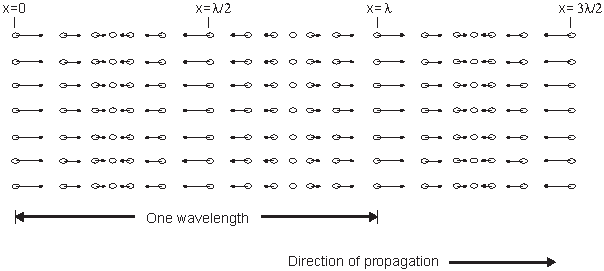
\includegraphics[width=\textwidth]{2_plane_wave_jensen-cropped.pdf}
	\caption[Particle displacement for a propagating ultrasound wave]{Particle displacement for a propagating ultrasound wave \cite{JensenUltrasoundBook}}
	\label{fig:2_planewave_jensen}
\end{figure}
\gls{us} is a technology that transmit sound wave with frequencies above the audible range (\qtyrange[range-units = single]{20}{20e3}{\hertz}) to mechanically vibrate matter. The particles in the medium would be at rest and distributed uniformly before any disturbance. The wave propagates as a disturbance and the particles oscillate around their mean position due to the presence of the ultrasonic wave. Typically the \gls{us} frequency band used in clinical settings are from \qtyrange[range-units = single]{1}{15}{\mega\hertz} \cite{Szabo_UltrasoundBook_2}. \Cref{fig:2_planewave_jensen} visualizes the propagation of a plane wave in matter. The oscillation occurs parallel to the wave's direction, making it longitudinal, and the disturbance will propagate with the variable $c$, which is determined by the medium and is given by \cref{eq:2_velocity_c}.
\begin{equation} \label{eq:2_velocity_c}
	c = \sqrt{\frac{1}{\rho_{0} \kappa_{S}}}
\end{equation}
Where $\rho_{0}$ is the mean density (\unit{\kilogram\per\meter\cubed}) and $\kappa_{S}$ is the \gls{adiabatic} compressibility (\unit{\meter\squared\per\newton}). Since in the majority of cases, the propagation of ultrasound is linear, it is assumed in this work. The acoustic pressure of the harmonic plane wave is expressed by \cref{eq:2_acoustic_pressure}
\begin{equation} \label{eq:2_acoustic_pressure}
	p(t,z)=p_{0} e^{j(\omega t - k z)}
\end{equation}
And propagates along the $z$-axis. $\omega$ is the angular frequency, $k$ is the wave number and is expressed by $k=\nicefrac{\omega}{c}=\nicefrac{2\pi}{\lambda}$, and $_{0}$ is the acoustic pressure amplitude. A spherical wave is expressed by \cref{eq:2_spherical_wave}
\begin{equation} \label{eq:2_spherical_wave}
	p(t,r)=p_{0} e^{j(\omega t - k r)}
\end{equation}
Where $r$ is radial distance, and is defined in a polar coordinate system. For each time instance, the acoustic pressure $p(t,r)$ is constant over a fixed radial position. In this scenario, the pressure amplitude is given by $p_{0}(r) = \nicefrac{k_{p}}{r}$, where $k_{p}$ is a constant since the energy of the outgoing wave must be constant.  Particle speed $u$ is dependent on the pressure caused by a wave expressed by \cref{eq:2_particle_speed}
\begin{equation} \label{eq:2_particle_speed}
	u = \frac{p}{Z}
\end{equation}
Where $Z$ is the characteristic acoustic impedance, defined as the ratio of acoustic pressure to particle speed at a given position in the medium and is expressed by \cref{eq:2_acoustic_impedance}.
\begin{equation} \label{eq:2_acoustic_impedance}
	Z = \rho_{0} c
\end{equation}

Characteristic acoustic impedance $Z$ is one of the most significant variables in the characterization of propagating plane waves. Reference values for density, speed of sound, and characteristic acoustic impedance can be seen in \cref{tab:2_density_tissue}.

\begin{table}[ht]
	\centering
	\caption[Approximate density, sound speed, and acoustic impedance of human tissue types]{Approximate density, sound speed, and acoustic impedance of human tissue types \cite{JensenUltrasoundBook}}
	\label{tab:2_density_tissue}
	\sisetup{range-phrase=--,range-exponents = combine}
	\begin{tblr}[]{ 
		colspec = {XSSS},
		row{1} = {guard,m,font=\small\bfseries},
		}
		\toprule
		Medium & {Density ($\rho_{0}$)\\\unit[per-mode = symbol]{\kilogram\per\meter\cubed}} & {Speed of sound ($c$)\\\unit[per-mode = symbol]{\meter\per\second}} & {\textbf{Acoustic impedance ($Z$)}\\\unit[per-mode = symbol]{\kilogram\per\meter\squared\per\second}} \\ \midrule
		Air             & 1.2     & 333            & 0.4e3       \\
		Blood           & 1.06e3    &    1566        &  1.66e6     \\
		Bone            & \numrange{1.38e3}{1.81e3}  &   \numrange{2070}{5350}       & \numrange{3.75e6}{7.38e6} \\
		Brain           &  1.03e3       & \numrange{1505}{1612}  & \numrange{1.55e6}{1.66e6} \\
		Fat             &  0.92e3  &  1446 & 1.33e6 \\
		Kidney          &  1.04e3  & 1567 & 1.62e6 \\
		Lung            &  0.4e3  &  650  & 0.26e6 \\
		Liver           &  1.06e3  &  1566  & 1.66e6 \\
		Muscle          &  1.07e3  & \numrange{1542}{1626} & \numrange{1.65e6}{1.74e6} \\
		Spleen          &  1.06e3  & 1566 & 1.66e6 \\
		DI				&  1e3  & 1480 & 1.48e6 \\ \bottomrule
	\end{tblr}
\end{table}

In the following sections, various acoustic wave phenomena will be briefly described.

\subsection{Scattering}
A wave propagating through a medium continues in the same direction until it encounters a new medium. When this occurs, a portion of the wave is transmitted into the new medium with a change in direction. Because the scattered wave is the result of several contributors, it is necessary to define it statistically. The amplitude distribution is Gaussian \cite{JensenUltrasoundBook} and can thus be fully described by its mean and variance. The mean value is zero because the dispersed signal is caused by variances in the acoustic characteristics in the tissue. The correlation between multiple data is what allows ultrasound to determine blood velocities. Because minor movements have a significant correlation, it is feasible to discover alterations in location by comparing sequential measurements of moving structures, such as blood cells. In medical ultrasound, only one transducer is used to transmit and receive, and only the backscattered signal is analysed. The power of the scattered signal is defined by the scattering cross-section, which in small cases means a uniform intensity $I_{i}$, and is expressed by \cref{eq:2_scatter_power}.
\begin{equation} \label{eq:2_scatter_power}
	P_{s} = I_{i} \sigma_{s c}
\end{equation}
Where $\sigma_{s c}$ is the scattering cross-section in square meters. The backscattering cross section is material dependant and determines the intensity of the scattering. If the dispersed energy is evenly emitted in all directions, the scattered intensity is given by \cref {eq:2_scatter_intensity}.
\begin{equation} \label{eq:2_scatter_intensity}
	I_{s} = \frac{P_{s}}{4 \pi R^{2}} = \frac{\sigma_{sc}}{4 \pi R^{2}} \cdot I_{i}
\end{equation}
Where $R$ is distance to the scattering region \cite{JensenUltrasoundBook}. This results in a spherical wave. A transducer with radius $r$ gives the power $P_{r}$, presuming the attenuation and focus is neglected, and is expressed by \cref{eq:2_transducer_r_power}.
\begin{equation} \label{eq:2_transducer_r_power}
	P_{r} = I_{s} \pi r^{2} = \sigma_{s c} \frac{r^{2}}{4 R^{2}} \cdot I_{i}
\end{equation}

The backscattering coefficient, which characterizes scattering from a volume of scatterers, is another measure of scattering strength. It is defined as the average received power per steradian volume of scatterers when flooded with plane waves of unit amplitude and the unit is \unit{1\per\centi\meter\steradian}. Backscattering coefficients in the blood are significantly lower than the backscattering coefficients from various tissue types. This poses a challenge when estimating blood flow close to tissue vessel walls \cite{ShungScattering1992,JensenUltrasoundBook}.

\subsection{Attenuation}
The ultrasonic wave will be reduced as it propagates through the tissue due to absorption and scattering. The attenuation in tissue is frequency dependent, with greater attenuation with increasing frequency. Because of absorption and dispersion, the ultrasonic wave will be attenuated as it travels through the tissue. The relationship between attenuation, distance travelled, and frequency is often linear. Attenuation in the tissue occurs as a result of both dispersion, which spreads energy in all directions, and absorption, which turns it into thermal energy. 

\begin{table}[ht]
	\centering
	\caption[Approximate attenuation values for human tissue]{Approximate attenuation values for human tissue
		\cite{JensenUltrasoundBook}}
	\label{tab:my_label}
	\sisetup{range-phrase=--,range-exponents = combine}
	\begin{tblr}[]{%
			colspec = {lS},
			row{1} = {guard, m, font=\small\bfseries},
		}
		\toprule
		Tissue & {Attenuation \\ $\unit[per-mode = symbol,inter-unit-product =\cdot]{\dB\per\mega\hertz\per\centi\meter}$ } \\ 
		\midrule
		Liver & \numrange{0.6}{0.9}{} \\
		Kidney & \numrange{0.8}{1}{} \\
		Spleen & \numrange{0.5}{1}{}\\
		Fat & \numrange{1}{2}{} \\
		Blood & \numrange{0.17}{0.24}{} \\
		Plasma & 0.01 \\
		Bone & \numrange{16}{23}{} \\
		\bottomrule
	\end{tblr}
\end{table}

The pressure of a wave propagating in $z$-direction decreases exponentially expressed by \cref{eq:2_attenuation_pressure}
\begin{equation} \label{eq:2_attenuation_pressure}
	p(z) = p(z=0) e^{-\alpha z}
\end{equation}
Where $p(z=0)$ is the pressure in the point of origin and $\alpha$ is the attenuation coefficient. The attenuation coefficient unit is \si{\neper\per\centi\meter} and, alternatively, \si{\dB\per\centi\meter} with the relationship described in \cref{eq:2_attenuation_coefficient}. 

\begin{subequations} \label{eq:2_attenuation_coefficient}
	\begin{align}
		\ensuremath{\alpha &= \frac{1}{z} \ln \frac{p(z=0)}{p(z)} \\
		\alpha( \si{\dB\per\centi\meter} ) &= 20 ( log_{10}e) \alpha ( \si{\neper\per\centi\meter}) = 8.68\alpha (\si{\neper\per\centi\meter})}
	\end{align}
\end{subequations}

The significance of absorption and scattering in ultrasonic attenuation in biological tissues is a point of contention. Scattering adds just a few per cent to attenuation in most soft tissues. As a result, it is fair to conclude that absorption is the primary mechanism of ultrasonic attenuation in biological tissues \cite{ShungUltrasound_Book}.

\subsection{Transducer}

\begin{figure}[ht]
	\centering
	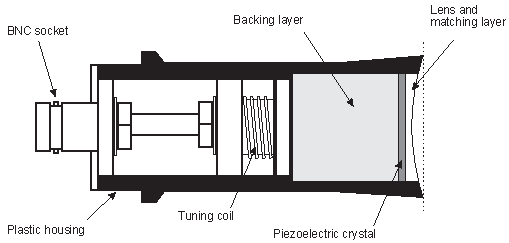
\includegraphics[width=.6\textwidth]{2_transducer_construction-cropped.pdf}
	\caption[Single element ultrasound transducer construction]{Single element ultrasound transducer construction \cite{JensenUltrasoundBook}}
	\label{fig:2_transducer_construction}
\end{figure}

A layperson knows transducers as speakers and microphones in the context of PA systems. In the case of medical \gls{us} it is the device that generates the acoustic pressure field, which is emitted into the tissue. The transducer has a piezoelectric crystal inside the housing. When excited, this crystal emits ultrasound waves toward flowing blood. The red blood cells will reflect a fraction of the emitted waves. These reflected waves are of a different frequency than the transmitted wave. If the red blood cells move away from the transducer, the frequency will be lower. If the red blood cells are moving towards the transducer, the frequency will be higher. This is caused by the \gls{doppler}. The reflected ultrasonic waves return to the crystal and are converted back into electrical signals. The single-element transducer shown in \cref{fig:2_transducer_construction} has a minimal imaging window and has to be mechanically manipulated to obtain a wide window, which is unfeasible for responsive high-frequency imaging. Thus, usually an array transducer is used. Various types of \gls{us} transducer exist with different strengths and weaknesses, shown in \cref{fig:2_transducer_types}. 

\begin{figure}[ht]
	\centering
	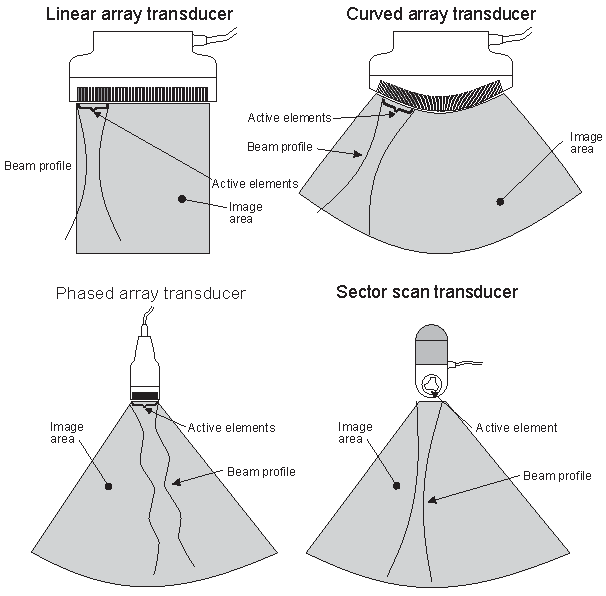
\includegraphics[width=.8\textwidth]{2_transducer_types-cropped.pdf}
	\caption[Transducer types for acquiring B-mode images]{Transducer types for acquiring B-mode images \cite{JensenUltrasoundBook}}
	\label{fig:2_transducer_types}
\end{figure}

\subsection{Doppler effect} \label{sec:doppler_effect}

\begin{figure}[ht]
	\centering
	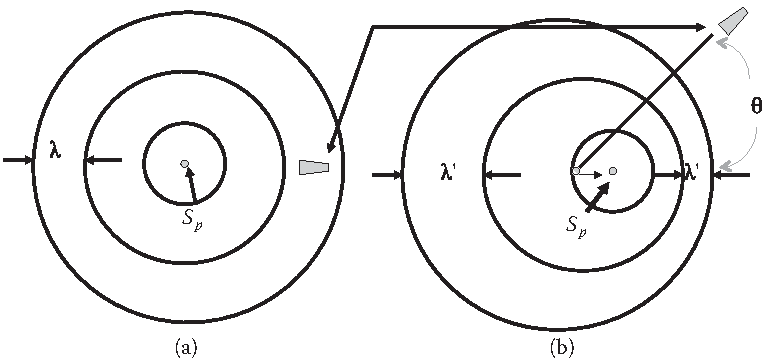
\includegraphics[width=.8\textwidth]{2_doppler_shung-cropped.pdf}
	\caption[Doppler effect diagram]{Doppler effect diagram. A stationary observer perceives a change in frequency of a wave generated by a moving source toward the observer as a result of a wavelength shift from $\lambda\ $ to $\lambda^{\prime}$. In (a), the source is still. In (b), the source is moving at a velocity $v$. \cite{ShungUltrasound_Book}}
	\label{fig:2_doppler_effect}
\end{figure}

The Doppler effect is a phenomena in which an observer perceives a shift in the frequency of sound emitted from a source when either the source or the observer is moving, or both are moving. The reason for the perceived change in frequency is visualised in \cref{fig:2_doppler_effect}. In diagram (a), the source $S_{p}$ is stationary and producing a spherical distribution pattern of the wave with the perceived frequency of the observer is given by $f=\nicefrac{c}{\lambda}$, where $c$ is the velocity of the wave in the medium and $\lambda$ is the wavelength. In diagram (b), the sound source is moving towards the right with a velocity $v$. The locomotion of the source changes the distribution pattern and causes a longer wavelength on the left, indicating a lower perceived frequency, and a shorter wavelength on the right, indicating a higher perceived frequency, both denoted as $\lambda^{\prime}$ in the diagram. In the case of the observer on the right side, the perceived frequency becomes \cref{eq:2_doppler_effect}.

\begin{equation} \label{eq:2_doppler_effect}
	f^{\prime} = \frac{c}{\lambda} = \frac{c}{\lambda - v T} = \frac{c}{(c-v)T} = \frac{c}{c-v}\cdot f_{0}
\end{equation}
And viceversa, on the left side, the perceived frequency becomes \cref{eq:2_doppler_effect2}.
\begin{equation} \label{eq:2_doppler_effect2}
	f^{\prime} = \frac{c}{c+v} \cdot f_{0}
\end{equation}
Where \todo{Hvad mangler her?}

This perceived difference between the frequency that is transmitted from the source $f_{0}$, and the perceived frequency $f^{\prime}$ is also called the Doppler frequency, $f_{d}$. When these connections are combined, the Doppler frequency for a source moving with velocity $v$ and an observer travelling with velocity $v^{\prime}$ is given by \cref{eq:2_doppler_moving}.
\begin{equation} \label{eq:2_doppler_moving}
	f_{d} = f^{\prime} - f = \left( \frac{c + v^{\prime}}{c - v}-1 \right)
\end{equation}
If both source and observer are moving with the same velocity, $v$, assuming $c\gg v$, the $v$ cancels out and the expression is reduced to \cref{eq:2_doppler_reduced}.
\begin{equation} \label{eq:2_doppler_reduced}
	f_{d} = \frac{2 v f}{c}
\end{equation}

If the velocity of the moving source is traveling with an incident angle $\theta$, the $v$ in \cref{eq:2_doppler_reduced} is replaced with $v (\cos\theta)$. This results in the expression found in \cref{eq:2_doppler_theta} and forms the basis for applied \gls{doppler} measurements.
\begin{equation} \label{eq:2_doppler_theta}
	f_{d} = \frac{2 v(\cos\theta) f}{c}
\end{equation}

The Doppler effect is used in ultrasonic Doppler devices used to image blood flow \gls{transcutaneous}ly. An ultrasonic transducer in these devices sends ultrasonic waves into a blood artery, and the scattered radiation from moving red cells is measured by either the same transducer or a second transducer. The Doppler frequency, which is determined by the velocity of red blood cells, is extracted using modern electronic demodulation techniques.

\section{Flow Physics}
\begin{figure}[ht!]
	\centering
	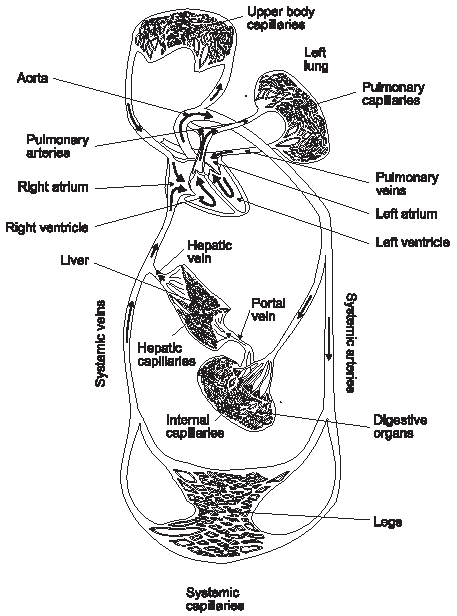
\includegraphics[width=\textwidth]{2_flow_circulatory_system_cropped.pdf}
	\caption[Circulatory system of the human body]{Circulatory system of the human body \cite{JensenUltrasoundBook}}
	\label{fig:2_circulatory_system}
\end{figure}

The flow physics of the human circulatory system are sophisticated, and numerous nonstationary flow patterns emerge. The human circulatory system takes care of transporting oxygen and nutrients to organs, as well as disposing of waste products produced by metabolism. It is possible because the blood within the circulatory system contains several smaller subcomponents, such as plasma and formed cellular elements that perform these vital functions. Initially, blood is discharged from the left ventricle of the heart through the aorta and travels to all areas of the body through multiple branches of the arterial tree. When blood flows through the arteries, it enters smaller channels known as arterioles. These arterioles lead to a network of tiny capillaries through which nutrients and waste materials are exchanged between the blood and the organs. The capillaries connect to form a network of venulae, which supply the veins and deliver blood back to the heart. This system, in its entirety, is called systemic circulation. A diagram of the circulatory system as described above can be seen in \cref{fig:2_circulatory_system}. In summary, when examining the elements that comprise the circulatory system, it consists of several components:
\begin{itemize}
	\item Heart, the primary organ of the circulatory system that maintains blood pressure and controls blood velocity.
	\item Blood, and its sub-components
	\begin{itemize}
		\item Plasma, which forms the primary volume and contains nutrients and formed cellular elements.
		\item Red and white blood cells, which carry oxygen and fight off infections, respectively.
		\item Platelets, which are also known as thrombocytes, have the function of clotting during blood vessel injury.
	\end{itemize}
	\item Blood vessels
	\begin{itemize}
		\item Arteries (and arterioles), transport oxygenised blood to organs and tissues at high pressure and velocity.
		\item Capillaries are thin but wide-ranging blood vessels that perform the exchange of matter between the circulatory system and tissue.
		\item Veins (and venules) carry blood back to the heart at low pressure and velocity.
	\end{itemize}
\end{itemize}

\subsection{Blood flow}
Blood flow is the amount of blood that goes through a blood vessel in a particular period of time, and has a complicated flow pattern due to its pulsing flow. Advanced analysis of haemodynamics is not within the scope of this report, so the explanation will be brief. The primary forces that determine the blood flow $F$ are the pressure difference across a blood vessel and vascular resistance. It is determined by Ohm's law as in \cref{eq:2_flow_ohms_law}.
\begin{equation} \label{eq:2_flow_ohms_law}
	F = \frac{\Delta P}{R}
\end{equation}
Where $\Delta P$ is the pressure difference across the blood vessel and $R$ is the vascular resistance. The pressure difference $\Delta P$ is calculated with \cref{eq:2_pressure_diff}.
\begin{equation} \label{eq:2_pressure_diff}
	\Delta P = P_{1}-P_{2}
\end{equation}
Where $P_{1}$ and $P_{2}$ are the blood pressures measured at each end of the blood vessel. Pressure has a significant importance on blood flow because an increase in arterial pressure not only increases the force that pushes blood through the capillaries but also expands the vessels, lowering vascular resistance.

\section{Devices}
\begin{figure}[ht]
	\centering
	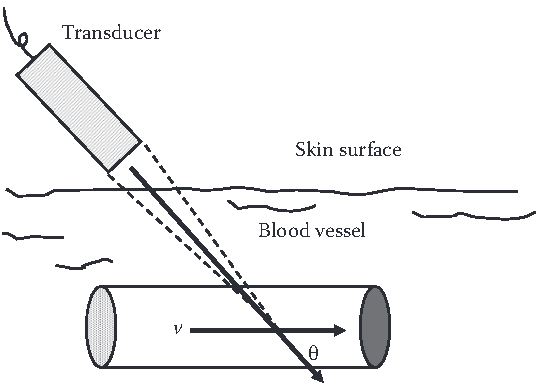
\includegraphics[width=.6\textwidth]{2_ultrasound_scan.pdf}
	\caption[Diagram of ultrasound wave transmitted and reaching blood vessel with incident angle $\theta$]{Diagram of \gls{us} wave transmitted and reaching blood vessel with incident angle $\theta$ \cite{ShungUltrasound_Book}}
	\label{fig:2_ultrasound_flow_scan}
\end{figure}

A device that measures the flowing of blood is called a flowmeter. Flowmeters may be used both inside and outside of vessels. One of the flowmeters that may be used outside the vessel to monitor flow is \gls{us}. \Cref{fig:2_ultrasound_flow_scan} depicts an ultrasonic wave of frequency $f$ insonifying a blood artery, resulting in an angle of $\theta$ relative to velocity $v$. For simplicity, it is assumed that blood flows in a vessel at a constant velocity $v$. The echoes returned are shifted in frequency as described in \cref{eq:2_doppler_theta} earlier in the chapter. The echoes scattered by blood after being insonified by an ultrasonic wave convey information about the velocity of blood flow. Blood flow measurements are often used in clinical settings to determine the status of blood vessels and organ functioning. The two commonly used fundamental techniques for ultrasound Doppler flow measurements are \gls{cw} and \gls{pw}. Both will be explained.

\subsection{Continuous-wave Flowmeter}
\begin{figure}[ht]
	\centering
	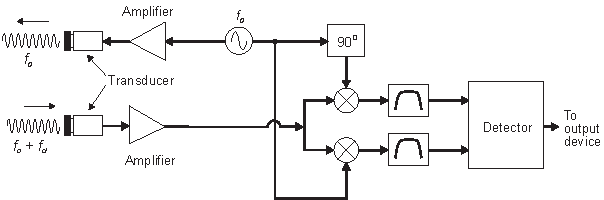
\includegraphics[width=\textwidth]{2_blockdiagram_cwdoppler.pdf}
	\caption[Block diagram of continuous-wave flowmeter]{Block diagram of \gls{cw} flowmeter \cite{JensenUltrasoundBook}}
	\label{fig:2_devices_cw}
\end{figure}
The earliest non-invasive cardiovascular diagnostic technologies relied heavily on \gls{cw} Doppler flowmeters. One of the earliest concepts for a device to estimate and study blood flow was proposed by \citeauthor{Satomura_CW}\cite{Satomura_CW} during the 1950s in Japan. To continuously transmit waves and receive signals from moving reflectors, the \gls{cw} flowmeter uses two transducers. \gls{cw} flowmeters use less sophisticated electronics than \gls{pw} flowmeters. A drawback to the \gls{cw} flowmeter is the lacking depth discrimination due to the continuous characteristic of this device type. A block diagram of a typical \gls{cw} flowmeter can be seen in \cref{fig:2_devices_cw}. The basic principles of the device are previously explained in \cref{sec:doppler_effect}, and the measurement of the device is described in \cref{eq:2_doppler_effect}. The device continuously emits an ultrasonic wave in the first transducer expressed as a function of time by \cref{eq:2_cw_tx} \cite{JensenUltrasoundBook}.
\begin{equation} \label{eq:2_cw_tx}
	e(t) = \cos (2\pi f_{0} t)
\end{equation}
While receiving the backscattered signal on the second transducer expressed by \cref{eq:2_cw_rx} \cite{JensenUltrasoundBook}.
\begin{align} \label{eq:2_cw_rx}
	r_{s}(t) &= a \cos \left( 2\pi f_{0} \alpha (t-t_{0}) \right) \\
	\alpha &\approx 1 - \frac{2 v_{z}}{c} \\
	\alpha t_{0} &\approx \frac{2 d_{0}}{c}
\end{align}
Where $v_{z}$ indicates the velocity in the $z$ direction. Applying the Fourier transform, the expression yields \cref{eq:2_cw_fourier}.
\begin{equation} \label{eq:2_cw_fourier}
	r_{s}(t)\cdot e^{j2\pi f_{0} t} \Longleftrightarrow R_{s}(f-f_{0})
\end{equation}
Where $R_{s}(f-f_{0})$ is the Fourier transform of $r_{s}(t)$. The received signal is then multiplied with a quadrature signal of frequency $f_{0}$ to find the Doppler frequency in \cref{eq:2_cw_quadrature}.
\begin{align} \label{eq:2_cw_quadrature}
	m(t) &= a \left[ \cos(2\pi f_{0} t) + j\sin (2\pi f_{0} t) \right] \cos (2\pi f_{0} \alpha (t-t_{0})) \\
	&= \frac{a}{2} \Bigl\{ \cos (2\pi f_{0} [ (1-\alpha) t- \alpha t_{0} ]) + \cos (2\pi f_{0} [ (1-\alpha) t- \alpha t_{0} ]) \\
	&\quad + j \sin (2\pi f_{0} [ (1-\alpha) t- \alpha t_{0} ]) + j \sin (2\pi f_{0} [(1-\alpha) t- \alpha t_{0} ]) \Bigr\} \nonumber
\end{align}

As is general for quadrature demodulation, the resulting signal contains the frequency components of the sum and difference of the emitted and received signals' frequencies shown in \cref{fig:2_demod_fd_frequency_domain}, where the signals are shown in time and frequency domains. 

\begin{figure}[ht]
	\centering
	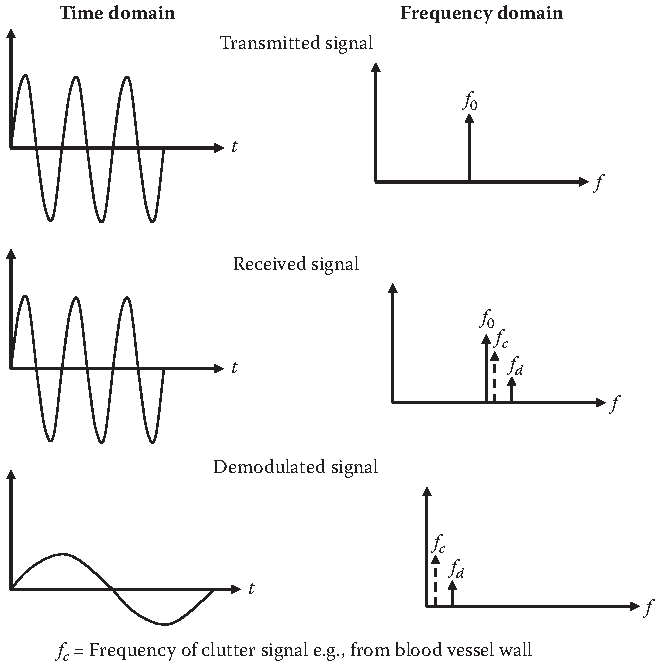
\includegraphics[width=.8\textwidth]{2_demod_fd_frequency_domain-cropped.pdf}
	\caption[Doppler signals in time and frequency domain showing demodulation effects]{Doppler signals in time and frequency domain showing demodulation effects \cite{ShungUltrasound_Book}}
	\label{fig:2_demod_fd_frequency_domain}
\end{figure}

Generally, a \gls{bp} filter is used on the demodulated signal to remove the high-frequency summed signal at twice the frequency of $f_{0}$. The filtered signal after the \gls{bp} filter is expressed by \cref{eq:2_cw_bp} and contains the Doppler shift of the emitted signal.
\begin{equation} \label{eq:2_cw_bp}
	m_{f}(t) \approx \frac{a}{2} e^{\left(j2\pi f_{0} \frac{2v_{z}}{c}t\right)} e^{\left( -j2\pi f_{0} \alpha t_{0} \right)}
\end{equation}
Where the second exponential term is the delay proportional to the time between transmission and receiving of the signal. The selected cutoff frequency is chosen to be much lower than the carrier frequency to remove the carrier wave. One issue with ultrasonic Doppler blood flow monitoring is that the blood vessels that generate large reflected echoes are also moving with a low velocity. These big, slow-moving echoes are referred to as clutter signals in Doppler nomenclature. The band pass filter's low-end cutoff frequency must be designed to minimize interference from these clutter signals. The design of this band pass filter in the low-frequency region, which serves the function of high pass, also known as a clutter rejection filter, has proven troublesome since the magnitude of clutter signals is many orders greater than that of blood and may obfuscate those from slow-moving blood. 

\begin{table}[ht]
	\centering
	\caption[Measured frequency shifts with a Doppler \qty{3}{\mega\hertz} transducer at various velocities at a \qty{45}{\degree} incident angle]{Measured frequency shifts with a Doppler \qty{3}{\mega\hertz} transducer at various velocities at a \qty{45}{\degree} incident angle \cite{JensenUltrasoundBook}}
	\label{tab:2_cw_frequency_shifts}
	\begin{tblr}[]{%
			colspec = {SS},
			row{1} = {guard, m, font=\small\bfseries},
			%vlines, hlines,
		}
		\toprule
		{Velocity $\left(v\right)$ \\ \unit[per-mode = symbol]{\meter\per\second}} & {Doppler frequency $\left(f_{d}\right)$ \\ \unit{\hertz} } \\ 
		\midrule
		0.01 & 28 \\
		0.1 & 276 \\
		0.5 & 1377 \\
		1 & 2755 \\
		2 & 5510 \\
		5 & 13770 \\
		\bottomrule
	\end{tblr}
\end{table}

Seen in \cref{tab:2_cw_frequency_shifts} is an example of measured Doppler frequencies using a \qty{3}{\mega\hertz} transducer using the method shown in \cref{fig:2_ultrasound_flow_scan}. Note that the measured frequencies are all within the audible range.

\subsection{Pulsed-wave Flowmeter}
\begin{figure}[ht]
	\centering
	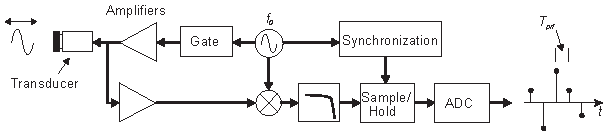
\includegraphics[width=\textwidth]{2_blockdiagram_pwdoppler.pdf}
	\caption[Block diagram of pulsed-wave flowmeter]{Block diagram of \gls{pw} flowmeter \cite{JensenUltrasoundBook}}
	\label{fig:2_devices_pw}
\end{figure}
The concept of a pulsed-wave flowmeter was proposed in \cite{Baker1970} and other related articles. This type of flowmeter is periodically changing from a transmitter to a receiver. In the transmit mode, the transducer emits a series of pulses. When in the receiving mode, the transducer is listening for the backscattered signal. A simplified block diagram can be seen in \cref{fig:2_devices_pw}. The movement of particles within the blood causes a displacement in the backscattered signal. These systems are commonly referred to as \enquote{Doppler systems} even though it is somewhat misleading. The effects of attenuation are also causing a shift in frequency of a higher magnitude than the velocity of particles in the blood. This is because the conventional Doppler effect is not the straightforward methodology that is applied to the analysis of the back-scattered signal. It is, in fact, an artefact. It is the shift in the location of the scatters that is observed, not the shift in the transmitted frequency. \Cref{fig:2_pw_sampling_displacement} shows the received signal after demodulation and filtering; the depth in tissue is fixed here, and the signals displayed on the left side of the figure are the result of a pulse sequence. Each line represents a single pulse, and each pulse is emitted at a pulse repetition frequency, $f_{\textup{prf}}$. Instead, on the right, the dotted line shows the sampled signal formed by taking into account the amplitude of each pulse after a specified time period.

\begin{figure}[ht]
	\centering
	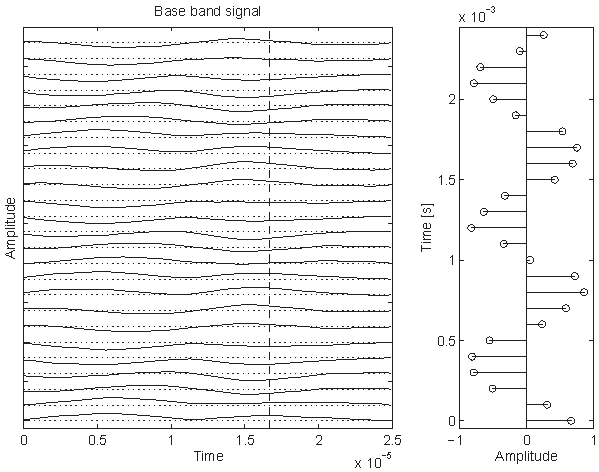
\includegraphics[width=.8\textwidth]{2_pw_pulse_sampling_displacement.pdf}
	\caption[Sampling for a gate pulsed wave system with a single range]{Sampling for a gate pulsed wave system with a single range. To depict the signals on the graph, a single pulse is emitted for each line, and the signals are displaced in amplitude. The sampled signal is displayed on the right. \cite{JensenUltrasoundBook}}
	\label{fig:2_pw_sampling_displacement}
\end{figure}


After the back-scattered signal is received it is multiplied by the centre frequency of the emitted pulse and filtered to remove the sum frequency \cite{JensenUltrasoundBook}. A \gls{adc} quantifies the signal for further signal processing. Referring to displacement \cref{fig:2_pw_sampling_displacement} again, the dashed vertical line represents the sample of each pulse that is taken. If sampling is done $T_{s}$ after pulse emission, the measurement depth is expressed by \cref{eq:2_pw_depth}.
\begin{equation} \label{eq:2_pw_depth}
	d_{0} = \frac{T_{s}c}{2}
\end{equation}
Hypothetically, if the velocity of stationary scatterers in blood was measured, a constant amplitude would be measured. A change in the sample value is observed when there is movement. Between two pulses, the scatterer movement is proportional to the velocity $v_{z}$ in the direction of the ultrasound beam. The time shift of $t_{s}$ is expressed as \cref{eq:2_pw_timeshift}.
\begin{equation} \label{eq:2_pw_timeshift}
	t_{s} = \frac{2v_{z}}{c}\cdot T_{\textup{prf}}
\end{equation}
Where $c$ is the speed of sound, and $T_{\textup{prf}}$ is the timespan between each pulse emission. Taking one sample from each line at a certain depth yields a sampled signal with a frequency proportional to the scatter velocity. Thus, if a sample is taken at the same depth for each line, resulting in a sinusoidal signal proportional in frequency to the scatter velocity \cite{Munk_Thesis} and that signal is expressed by \cref{eq:2_pw_scatter_velocity_a,eq:2_pw_scatter_velocity_b}.
\begin{subequations}
	\begin{align} 
		r(i) &= a(i) \sin \left( 2\pi f_{p} T_{\textup{prf}} \cdot i \right) \label{eq:2_pw_scatter_velocity_a} \\
		f_{p} &= \frac{2 v_{z}}{c} f_{0} \label{eq:2_pw_scatter_velocity_b}
	\end{align}
\end{subequations}
Where $a(i)$ is the amplitude, $f_{0}$ is the emitted frequency, and $\theta$ is the phase factor in the depth of interest. \todo{Hvor er $\theta$ i udtrykket? Omskriv fra Jensen2012} This technique improved the accuracy of the investigations of blood vessels and facilitated the display of velocity profiles. Furthermore, by employing two transducers or a multi-element transducer, duplex mode imaging (displaying both a B-mode picture and a blood velocity estimate) became feasible. Two-transducer systems are no longer utilised since it is easier to create a duplex picture with a multi-element transducer. 

\section{Blood Velocity Estimation}
Once a backscattered signal is received, estimation of velocity can be obtained with multiple methods. In this section the most common methods to estimate blood velocity are mentioned with their strengths and limitations. 
\subsection{Spectral estimation}
\begin{figure}[htbp]
	\centering
	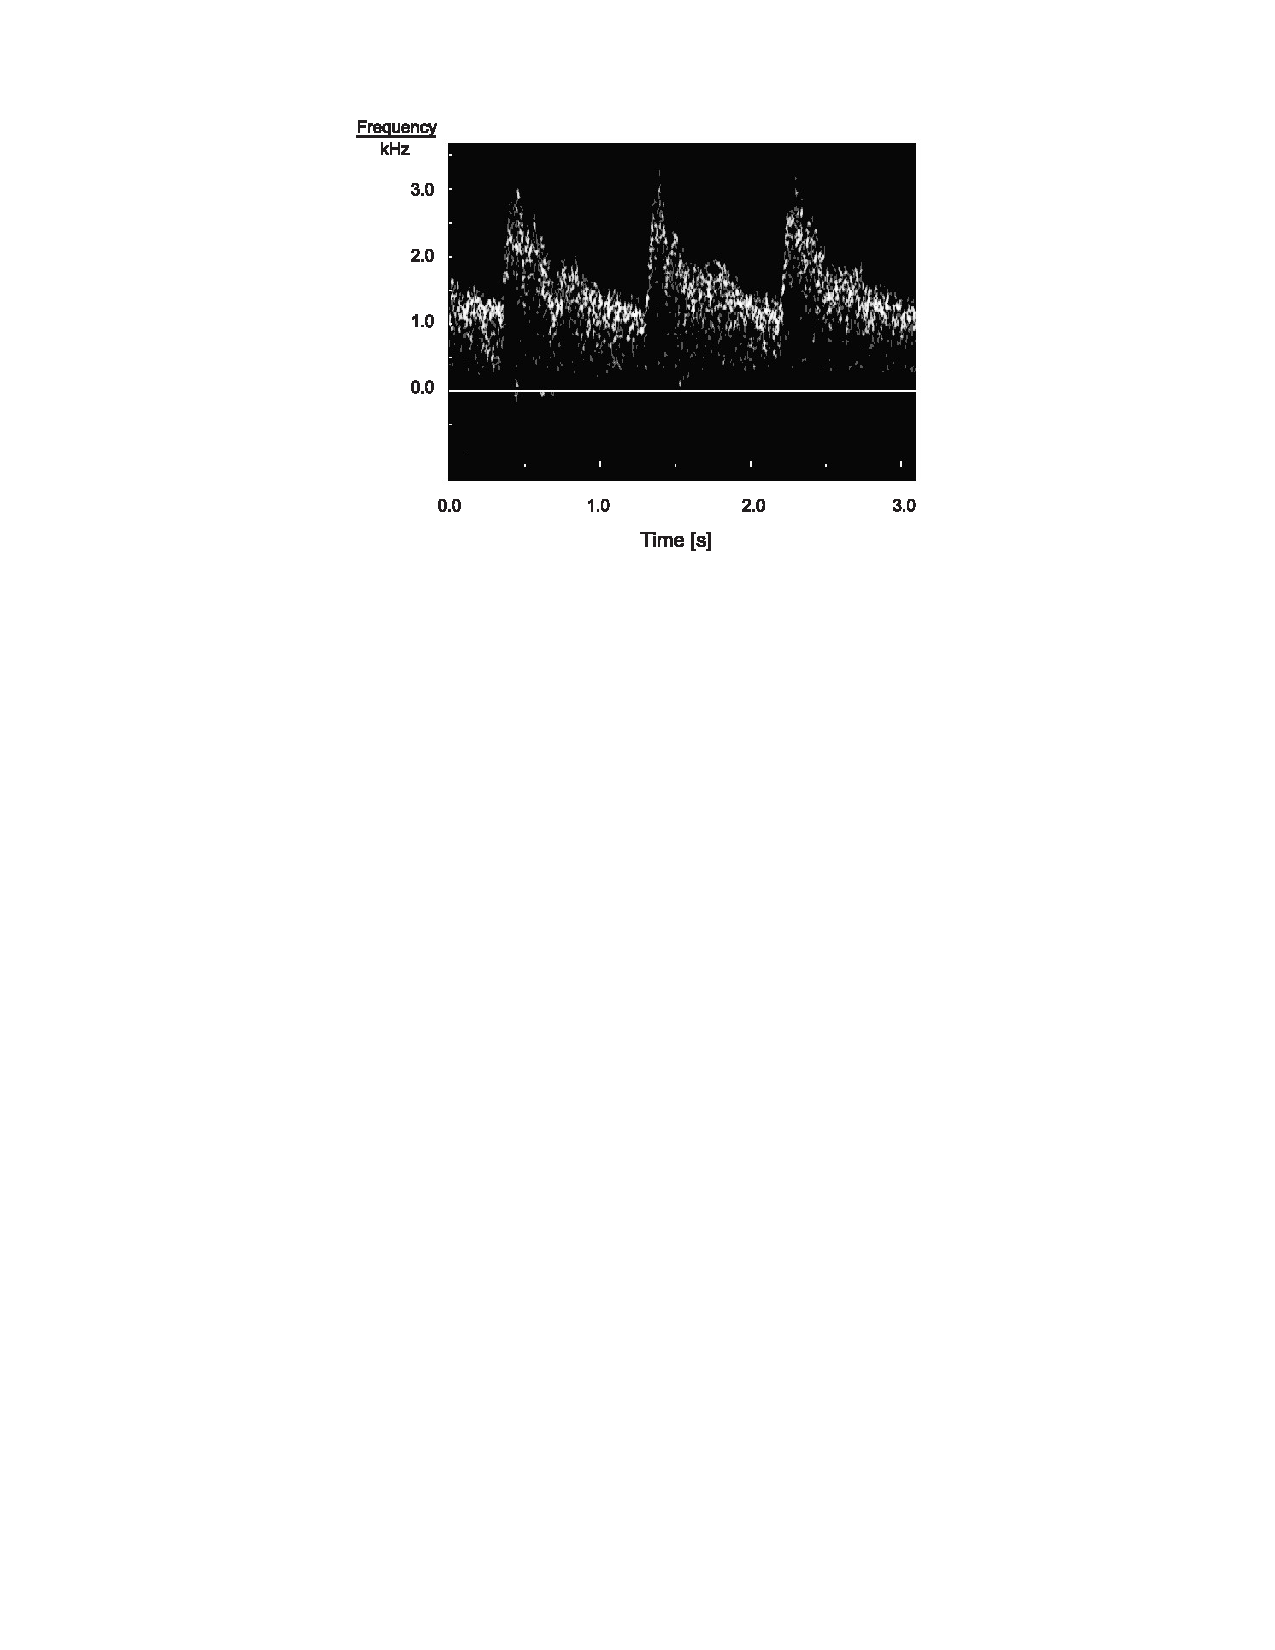
\includegraphics[width=.8\textwidth]{Figures/2_estimation_sonogram_cph.pdf}
	\caption{Arterial sonogram with time-frequency and Doppler shift \cite{JensenUltrasoundBook}}
	\label{fig:2_estimation_sonogram_cph}
\end{figure}

Given that the frequency volume of the received signal is similar to the blood's velocity distribution, the Fourier transform of the received signal can be used to obtain velocity. The spectrogram, usually erroneously known as the Doppler spectrum, can be created by saving the \gls{psd} together. The \gls{psd} is calculated for each of the components that make up the received signal in order to accomplish this. A quadrature demodulated signal is used to display both positive and negative frequencies. When these spectra are shown side by side, the evolution of the velocity distribution can then be seen. The ultrasonography of an artery is displayed in \cref{fig:2_estimation_sonogram_cph}. 
%	\chapter{Introduction}
%	\noindent
%	Cognitive radio (CR), a key technology of resource-efficient wireless communications, can be employed to solve the problem of frequency resource shortage. However, due to the uncertainty of the secondary users' (SUs') usage of frequency band, the original CR has failed to gain sufficient interests. Recently, a new paradigm termed cooperative cognitive radio networks (CCRNs) has been proposed \cite{FD1}-\cite{ML1}...
%
%	There ...

	\chapter[Related Works and Contributions of this Dissertation]{Related Works and \\ Contributions of this Dissertation}

	\section{Quantum Communication}

	There have been extensive studies on cognitive radio in recent years. To enhance the performance gain of original cognitive radio networks (CRNs), leveraging cooperative diversity has attracted a lot of attention \cite{SOCA1}...

	\subsection{Examples}


	\section{Applications of Quantum Communication}

	Despite its potential to improve the throughput, spatial domain diversity was not fully considered in the studies of original CCRNs. Utilizing the spatial domain for the communications, the concept of MIMO has been adopted in many cases to increase the wireless capacity \cite{EF1,FD2}...


	\chapter{Proposed Architecture and Its Application}

	\section{Proposed Architecture}

	Let us consider an MIMO-CCRN with one PL and one SL. Each PU has one legacy antenna and each SU has two STAR antennas. The duration of one communication time frame is divided into two phases \cite{RVP2,ML2} ...
	%%
	%% 표 삽입 예시
	%% Example. how to insert table
	%%
	\begin{table}[t]
		\caption[Enter the caption title here]{Energy stability $E$ (eV) per molecule of all meta-stable
			isomer states of C$_{60}$ opening process for forming the (5,5) cap.
			In the SW-I and SW-II, both ferromagnetic (Ferro) and paramagnetic (Para)
			spin configurations are obtained, whereas only non-magnetic configuration
			is obtained in the BF, SW-III, and CAP(5,5).
			$M$ is total magnetization $n_{\rm up}$-$n_{\rm down}$ in unit of $\mu_B$, where
			$n_{\rm up(down)}$ is the number of up (down) spins.
		}
		\label{mag-tab1}
		\begin{center}
			\begin{tabular} {ccccccccccc}
				\hline\hline
				& & BF &\multicolumn{2}{c}{SW-I}&&\multicolumn{2}{c}{SW-II}&SW-III&CAP&\\
				\cline{4-5} \cline{7-8}
				&               &   &  Para & Ferro &&   Para &  Ferro &      &      &\\
				\hline
				& $E$ (eV)      & 0 & 7.796 & 7.832 && 10.418 & 10.408 & 11.5 & 13.2 &\\
				& $M$ ($\mu_B$) & 0 &     0 &  1.94 &&      0 &   2.06 &    0 &    0 &\\
				\hline\hline
			\end{tabular}
		\end{center}
	\end{table}

	%%
	%% 그림 삽입 예시
	%% Example. how to insert graph
	%%
	%% Note. 가급적 \includegraphics 명령을 사용하십시오.
	%% Recommen : Use \includegraphics to insert graph.
	%%
	\begin{figure}[t]
		\centerline{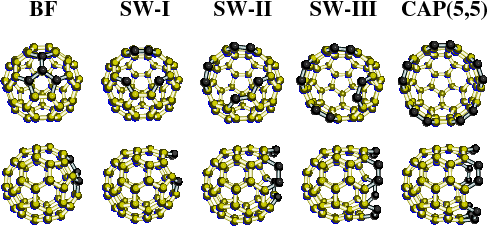
\includegraphics[width=12.5cm]{sample-fig1}}
		\caption[Enter the caption title here]{ Ball-and-stick models of meta-stable isomers in
			cage opening process from a C$_{60}$ buckminsterfullerene
			to a (5,5) capsule. We name them BF and CAP(5,5).
			Depending on the number of the Stone-Wales (SW) transformation,
			we call the intermediate isomers with SW-I, SW-II, and SW-III.
			Highlighted atoms are undercoordinated except BF.
		} \label{mag-fig1}
	\end{figure}

	\section{Application}

	The achievable rates can be calculated by finding the statistics of the five signals transmitted that maximize the mutual information between $s_{t,XY}$ and $y_{t,XY}$ for $(X,Y)=(T,C), (C,N)$, and $(N,C)$ when $t=1$, and $(X,Y)=(C,R), (C,N)$, and $(N,C)$ when $t=2$ \cite{SOCA2,EF2}...


	\chapter{Concluding Remark}

	We have proposed a novel FD MIMO-CCRN framework providing a reasonable performance improvement compared with the conventional MIMO-CCRN framework...
	%%
	%% 참고문헌 시작
	%% bibliography
	%% It can be changed but should include sufficient information.
%	\begin{thebibliography}{00}
%
%		\bibitem{FD1} 박상우, \underline{동시 송수신 안테나를 두 개 쓰는 협력 인지 무선통신망에 알맞은 전 이중 통신}, 한국과학기술원 석사 학위 논문, 2016.
%
%		\bibitem{RVP1} 송익호, 박철훈, 김광순, 박소령, \underline{확률변수와 확률과정}, 자유아카데미, 2014.
%
%		\bibitem{ML1} 송익호, 안태훈, 민황기, \underline{인지 무선에서의 광대역 주파수 검출 방법 및 장치}, 특허등록번호 10-1494966, 2015년 2월 12일.
%
%		\bibitem{SOCA1} 호우위시, 이원주, 이승원, 안태훈, 이선영, 민황기, 송익호, “선형 판별 분석에서 부류안 분산 행렬의 영 공간 재공식화,” \underline{한국통신학회 2012년도 추계종합학술발표회}, 대한민국 고려대학교, 242-243쪽, 2012년 11월.
%
%		\bibitem{EF1} 민황기, 안태훈, 이승원, 이성로, 송익호, “비간섭 전력 부하 감시용 고차 적률 특징을 갖는 전력 신호 인식,” \underline{한국통신학회논문지}, 제39C권, 제7호, 608-614쪽, 2014년 7월.
%
%
%
%		\bibitem{FD2} S. Park, \textit{Full-Duplex Communication for Cooperative Cognitive Radio Networks with Two Simultaneous Transmit and Receive Antennas}, Master Thesis, Korea Adv. Inst. Science, Techn., Daejeon, Republic of Korea, 2016.
%
%		\bibitem{RVP2}  I. Song, J. Bae, and S. Y. Kim, \textit{Advanced Theory of Signal Detection: Weak Signal Detection in Generalized Observations}, Springer-Verlag, 2002.
%
%		\bibitem{ML2} I. Song, T. An, and J. Oh, \textit{Near ML decoding method based on metric-first search and branch length threshold,} registration no. US 8018828 B2, Sep. 13, 2011, USA.
%
%		\bibitem{SOCA2} H.-K. Min, T. An, S. Lee, and I. Song, “Non-intrusive appliance load monitoring with feature extraction from higher order moments,” in \textit{Proc. 6th IEEE Int. Conf. Service Oriented Computing, Appl.,} Kauai, HI, USA, pp. 348-350, Dec. 2013.
%
%		\bibitem{EF2} I. Song and S. Lee, “Explicit formulae for product moments of multivariate Gaussian random variables,” \textit{Statistics, Probability Lett.,} vol. 100, pp. 27-34, May 2015.
%
%
%	\end{thebibliography}
%
%

	%%
	%% 감사의 글 시작
	%% Acknowledgement
	%%
	% @command acknowledgement 감사의글
	% @options [1 | 2 | 3 |4 ]
	% - 1 : 본문과 감사의 글이 둘 다 한글일 때  | 2 : 본문은 한글인데 감사의 글이 영어일 때 | 3 :  본문과 감사의 글이 둘 다 영어일 때  | 4 : 본문은 영어인데 감사의 글이 % 한글일 때
	%% It is optional.

	\acknowledgment[4]
	언제나 저를 바른 길로 이끌어 주시는 송익호 교수님께 큰 고마움을 느낍니다.
	끝으로 오늘의 제가 있을 수 있도록 사랑으로 키워 주신 가족들에게 감사드립니다.
	저의 이 작은 결실이 그분들께 조금이나마 보답이 되기를 바랍니다.

	%%
	%% 약력 시작
	%% Curriculum Vitae
	%%
	% @command curriculumvitae 이력서
	% @options [1 | 2 | 3 |4 ]
	% - 1 : 본문과 약력이 둘 다 한글일 때  | 2 : 본문은 한글인데 약력이 영어일 때 | 3 :  본문과 약력이 둘 다 영어일 때  | 4 : 본문은 영어인데 약력이 한글일 때
	%% It is optional and you can change form of this in the class file if you want.
	\curriculumvitae[4]

	% @environment personaldata 개인정보
	% @command     name         이름
	%              dateofbirth  생년월일
	%              birthplace   출생지
	%              domicile     본적지
	%              address      주소지
	%              email        E-mail 주소
	% - 위 6개의 기본 필드 중에 이력서에 적고 싶은 정보를 입력
	% input data only you want
	\begin{personaldata}
		\name       {힌릭스 예폐}
		\dateofbirth{1991}{07}{22}
		\birthplace {Aarhus}
		\address    {}
	\end{personaldata}

	% @environment education 학력
	% @options [default: (none)] - 수학기간을 입력
	\begin{education}
		\item[2008. 3.\ --\ 2010. 2.] 고등학교 (2년 수료)
		\item[2010. 2.\ --\ 2014. 2.] 한국과학기술원 물리학과 (학사)
		\item[2014. 3.\ --\ 2016. 2.] 한국과학기술원 전기및전자공학부 (석사)
	\end{education}

	% @environment career 경력
	% @options [default: (none)] - 해당기간을 입력
	\begin{career}
		\item[2015. 3.\ --\ 2016. 2.] 한국과학기술원 전기및전자공학부 조교
	\end{career}

	% @environment activity 학회활동
	% @options [default: (none)] - 활동내용을 입력
	%%    \begin{activity}
		%%        \item J. Choi, \textbf{Yong-Hyun Kim}, K.J. Chang, and D. Tomanek,
		%%             \textit{Occurrence of itinerant ferromagnetism in C/BN superlattice
			%%             nanotubes}, 5th Asian Workshop on First-Principles Electronic
		%%             Structure Calculations, Seoul (Korea), October., 2002.
		%%    \end{activity}

	% @environment publication 연구업적
	% @options [default: (none)] - 출판내용을 입력
	\begin{publication}
		%\item \textbf{Yong-Hyun Kim}, J. Choi, K.J. Chang, and D. Tomanek,
		%     \textit{Magnetic instability in partly opened C$_{60}$ isomers},
		%     in preparation.
		\item H.-K. Min, Y. Hou, {\bf S. Park}, and I. Song,
		``A computationally efficient scheme for feature extraction with kernel discriminant analysis,"
		\textit{Patt. Recogn.}, vol.~50, no.~2, pp.~45-55, Feb. 2016 (to be published).
	\end{publication}

	\label{paperlastpagelabel}     % <-- 추가 부분: 마지막 페이지 위치 지정
	%% 본문 끝
\end{document}
